

\begin{frame}{Coset Quandles}
 \textsc{Magma} uses the Todd-Coxeter coset enumeration algorithm.
\begin{algorithm}[H]
\caption{Coset Quandle Construction}\label{alg:coset}
\DontPrintSemicolon
\SetKwData{Set}{$L$}\SetKwData{Map}{$\phi$}\SetKwData{Graph}{$G(\cdot)$}\SetKwData{GraphNL}{$G(\mathcal{N}_L)$}
\SetKwFunction{LeftTransversal}{LeftTransversal}
\SetKwInOut{Input}{Input}\SetKwInOut{Output}{Output}\SetKwInOut{Return}{Return}
\Input{Group $G$, $f \in \text{Aut}(G)$, $H \leq \{x \in G : f(x) = x\}$}
\Output{$\mathcal{Q}_{\text{Hom}}(G,H,f)$}
\BlankLine
\BlankLine
\tcc{\LeftTransversal{$G,H$} returns an indexed set of elements $L = (l_i)_{i \in \{1,\dots,n\}}$ forming a left transversal for G over H; and the corresponding transversal mapping $\phi : G \to L\quad g \mapsto l_i$ such that $g\in l_iH$, for any $g \in G$.}
\Set, \Map $\leftarrow$ \LeftTransversal{$G, H$}\;

\tcc{Define the quandle operation by its functional graph \Graph}
\Graph $\leftarrow$ $\{((x,y), \Map(xf(x^{-1}y))) : x,y \in \Set\}$\;
\Return{$\textbf{A} = (\Set,\cdot)$}
\end{algorithm}

\end{frame} 

\begin{frame}{$Inn(Q)$ and checking $Dis_\alpha \leq Dis^\alpha$}

Transitive: $\forall x,y \in X\quad \exists g \in Inn(Q)\quad g(x)=y$.
\par\noindent\rule{0.7\textwidth}{0.4pt}
\begin{lemma}
Let $Q$ be a connected quandle, $\alpha$ a block system of $Inn(Q)$ and consider $[a_0]\in \alpha$ for some $a_0\in Q$. Define $A = \{ L_xL_{a_0}^{-1} : x \in [a_0]\} \subset \text{Dis}_\alpha(Q)$.
\[\textsf{If} \quad A \subset \text{Dis}^\alpha(Q) \quad \textsf{then} \quad \text{Dis}_\alpha(Q) \subset \text{Dis}^\alpha(Q)\]
% \{ L_xL_y^{-1} :  x~\alpha~y\}
\end{lemma}

\end{frame} 
\begin{frame}{Proof}
\small
\begin{proof}

% Now one has to check that $A\subset \text{Dis}^\alpha(Q)$; % - so now one has to verify that $\forall h \in A\quad h(x)\alpha x$ for every $x\in Q$. 
For any element $h\in A$ and $x\in Q$, either $h(x)\in [x]_\alpha$ and so $\forall y \in [x]_\alpha\quad h(y)\in[x]_\alpha$(case 1) \emph{or} $h(x)\notin [x]_\alpha$ and so $\forall y \in [x]_\alpha \quad h(y)\notin [x]_\alpha$(case 2). In case 2, $h \notin Dis^\alpha(Q)$ so $A \not\subset Dis^\alpha(Q)$ and $\pi$ is not added to \textsf{Congruences}. Case 1 justifies checking only a representative for each block. If case 1 holds for any $h \in A$, then $A \subset Dis^\alpha(Q)$.\newline
Therefore, assume that $A \subset Dis^\alpha(Q)$.\newline
Given that $[a_0]_\alpha$ is a block, $\forall x \in Q\quad \exists h\in Dis^\alpha(Q)\quad [x]_\alpha = h([a_0]_\alpha)$.\newline
For any $x~\alpha~y\in Q$, there exists $x_0,y_0\in [a_0]_\alpha$ and $h\in Dis(A)$ such that $x=h(x_0)$ and $y=h(y_0)$.
\begin{center}
    \begin{tabular}{ccl}
        $L_xL_y^{-1}$ & $=$ & $L_{h(x_0)}L_{h(y_0)}^{-1}$\\
         & $=$ & $hL_{x_0}h^{-1}hL_{y_0}^{-1}h^{-1}$\\
         & $=$ & $hL_{x_0}L_{y_0}^{-1}h^{-1}$\\
         & $=$ & $h\underbrace{L_{x_0}L_{a_0}^{-1}}_{\in \text{Dis}^\alpha}\underbrace{L_{a_0}L_{y_0}^{-1}}_{ \in \text{Dis}^\alpha}h^{-1} \in \text{Dis}^\alpha$\\
    \end{tabular}
\end{center}


\end{proof}
\end{frame}
\begin{frame}{Unarifying a binary operation}

The ``unarification" of a binary operation:

\[
\begin{bNiceMatrix}[left-margin = 6pt, right-margin = 6pt] 
\Block[draw=darkred, line-width = 2pt]{1-3}{}\Block[tikz={line width = 4pt, fill = green2, draw = white}]{*-1}{}a & \Block[tikz={line width = 4pt, fill = green2, draw = white}]{*-1}{}c & \Block[tikz={line width = 4pt, fill = green2, draw = white}]{*-1}{}b \\
\Block[draw=darkred, line-width = 2pt]{1-3}{}c & b & a \\
\Block[draw=darkred, line-width = 2pt]{1-3}{}b & a & c \\
\end{bNiceMatrix}
\]
\[\begin{bNiceMatrix}[left-margin = 6pt, right-margin = 6pt] 
\Block[draw=darkred, line-width = 2pt]{1-3}{}a & c & b 
\end{bNiceMatrix}
\begin{bNiceMatrix}[left-margin = 6pt, right-margin = 6pt] 
\Block[draw=darkred, line-width = 2pt]{1-3}{}c & b & a 
\end{bNiceMatrix}
\begin{bNiceMatrix}[left-margin = 6pt, right-margin = 6pt] 
\Block[draw=darkred, line-width = 2pt]{1-3}{}b & a & c 
\end{bNiceMatrix}
\begin{bNiceMatrix}[left-margin = 6pt, right-margin = 6pt] 
\Block[tikz={line width = 4pt, fill = green2, draw = white}]{1-3}{}a & c & b
\end{bNiceMatrix}
\begin{bNiceMatrix}[left-margin = 6pt, right-margin = 6pt] 
\Block[tikz={line width = 4pt, fill = green2, draw = white}]{1-3}{}c & b & a
\end{bNiceMatrix}
\begin{bNiceMatrix}[left-margin = 6pt, right-margin = 6pt] 
\Block[tikz={line width = 4pt, fill = green2, draw = white}]{1-3}{}b & a & a
\end{bNiceMatrix}\]
\[\begin{bNiceMatrix}[left-margin = 6pt, right-margin = 6pt] 
a & c & b 
\end{bNiceMatrix}
\begin{bNiceMatrix}[left-margin = 6pt, right-margin = 6pt] 
c & b & a 
\end{bNiceMatrix}
\begin{bNiceMatrix}[left-margin = 6pt, right-margin = 6pt] 
b & a & c 
\end{bNiceMatrix}\]



\[
\begin{bNiceMatrix}[left-margin = 6pt, right-margin = 6pt] 
\Block[draw=darkred, line-width = 2pt]{1-3}{}\Block[tikz={line width = 4pt, fill = green2, draw = white}]{*-1}{}a & \Block[tikz={line width = 4pt, fill = green2, draw = white}]{*-1}{}b & \Block[tikz={line width = 4pt, fill = green2, draw = white}]{*-1}{}c \\
\Block[draw=darkred, line-width = 2pt]{1-3}{}a & b & c \\
\Block[draw=darkred, line-width = 2pt]{1-3}{}a & b & c \\
\end{bNiceMatrix}
\]
\[\begin{bNiceMatrix}[left-margin = 6pt, right-margin = 6pt] 
\Block[draw=darkred, line-width = 2pt]{1-3}{}a & b & c 
\end{bNiceMatrix}
\begin{bNiceMatrix}[left-margin = 6pt, right-margin = 6pt] 
\Block[draw=darkred, line-width = 2pt]{1-3}{}a & b & c 
\end{bNiceMatrix}
\begin{bNiceMatrix}[left-margin = 6pt, right-margin = 6pt] 
\Block[draw=darkred, line-width = 2pt]{1-3}{}a & b & c 
\end{bNiceMatrix}
\begin{bNiceMatrix}[left-margin = 6pt, right-margin = 6pt] 
\Block[tikz={line width = 4pt, fill = green2, draw = white}]{1-3}{}a & a & a
\end{bNiceMatrix}
\begin{bNiceMatrix}[left-margin = 6pt, right-margin = 6pt] 
\Block[tikz={line width = 4pt, fill = green2, draw = white}]{1-3}{}b & b & b
\end{bNiceMatrix}
\begin{bNiceMatrix}[left-margin = 6pt, right-margin = 6pt] 
\Block[tikz={line width = 4pt, fill = green2, draw = white}]{1-3}{}c & c & c
\end{bNiceMatrix}\]

\[\begin{bNiceMatrix}[left-margin = 6pt, right-margin = 6pt] 
a & b & c 
\end{bNiceMatrix}
\begin{bNiceMatrix}[left-margin = 6pt, right-margin = 6pt] 
a & a & a
\end{bNiceMatrix}
\begin{bNiceMatrix}[left-margin = 6pt, right-margin = 6pt] 
b & b & b
\end{bNiceMatrix}
\begin{bNiceMatrix}[left-margin = 6pt, right-margin = 6pt] 
c & c & c
\end{bNiceMatrix}\]




\end{frame}
\tiny
\begin{frame}{Principal Congruence - Ralph Freese}
    \begin{algorithm}[H]

\DontPrintSemicolon
\caption{Principal congruence generated by pair $x,y$ - \texttt{Cg(\textsf{L}$, x, y$)}}

\SetKwData{true}{true}
\SetKwData{false}{false}
\SetKwData{unary}{UnaryOperations}
\SetKwData{f}{f}
\SetKwData{x}{x}
\SetKwData{y}{y}
\SetKwData{z}{z}
\SetKwData{t}{t}
\SetKwData{pairs}{Pairs}
\SetKwData{pair}{(x,y)}
\SetKwArray{partition}{Partition}
\SetKwArray{ls}{L}

\SetKwFunction{dequeue}{Dequeue}
\SetKwFunction{enqueue}{Enqueue}
\SetKwFunction{queue}{Queue}
\SetKwFunction{join}{JoinBlocks}
\SetKwFunction{root}{Root}

\SetKwInOut{Input}{Input}\SetKwInOut{Output}{Output}\SetKwInOut{Return}{Return}

\pairs $\leftarrow$ \queue{$\{(x,y)\}$}\;
\partition $\leftarrow$ $[-1_1, -1_2, \dots, -1_n]$\;
\tcc{\join{P, a, b} joins the blocks of partition P containing a and b}
\partition $\leftarrow$ \join{\partition, $x$, $y$}\;
\While{\pairs $\neq$ \queue{$\emptyset$}}{
    \pair $\leftarrow$ \dequeue{\pairs}\;
    \For{\f $\in$ \ls}{
        \tcc{\root{P, a} returns the root of the block in $P$ in which $a$ is.}
    \z $\leftarrow$ \root{\partition,\f{\x}}\;
    \t $\leftarrow$ \root{\partition,\f{\y}}\;
    \If{\z $\neq$ \t}{
        \partition $\leftarrow$ \join{\partition, \z, \t}\;
        \pairs $\leftarrow$ \enqueue{\pairs, $(\z,\t)$}\;
    }
    }
}
\Return{\partition}
\normalsize
The principal congruence for a pair $(x,y)$ is the smallest congruence such that that $x$ and $y$ are in the same equivalence class. 
\end{algorithm}

\end{frame}
\begin{frame}{How does Freese's expanded algorithm work?}
\normalsize
    \begin{enumerate}
        \item Unarify the quandle.
        \item Loop over $Q\times Q$ and use Freese's algorithm to compute all the principal congruences of the quandle and add them to the list of all congruences.
        
        \item Take a \textbf{principal} congruence and an item in the list of \textbf{all} congruences and, if the principal congruence is not contained in the congruence it is being joined with, join them and add the result to the list of all congruences. 
        \item Stop the process once no new congruence shows up.
    \end{enumerate}
\end{frame}

\begin{frame}{Automorphisms - Algorithm}
\normalsize
\begin{columns}
\begin{column}{0.45\textwidth}
\begin{definition}[\emph{Normalizer}]

Let $H$ be a group and $Y \subseteq G$.\newline
\[N_H(Y) = \{ h \in H : hYh^{-1} = Y\}\]
\end{definition}

\end{column}
\begin{column}{0.5\textwidth}

\begin{lemma}
Let $h : Q \to Q$.
\[h \in Aut(Q) \implies hL_xh^{-1} = L_{h(x)}\]
\end{lemma}
\end{column}
\end{columns}
\begin{center}
\begin{theorem}
Let $h : Q \to Q$.
\[h \in Aut(Q) \implies h \in N_{S_X}(Inn(Q))\]
\end{theorem}
    \textcolor{darkred}{\fbox{We do not need $\mathbf{n!}$ permutations, only $|N_{S_X}(Inn(Q))|$.}} 
\end{center}
\end{frame}

\begin{frame}{Applications 1/3}
\begin{figure}[H]
    \centering
    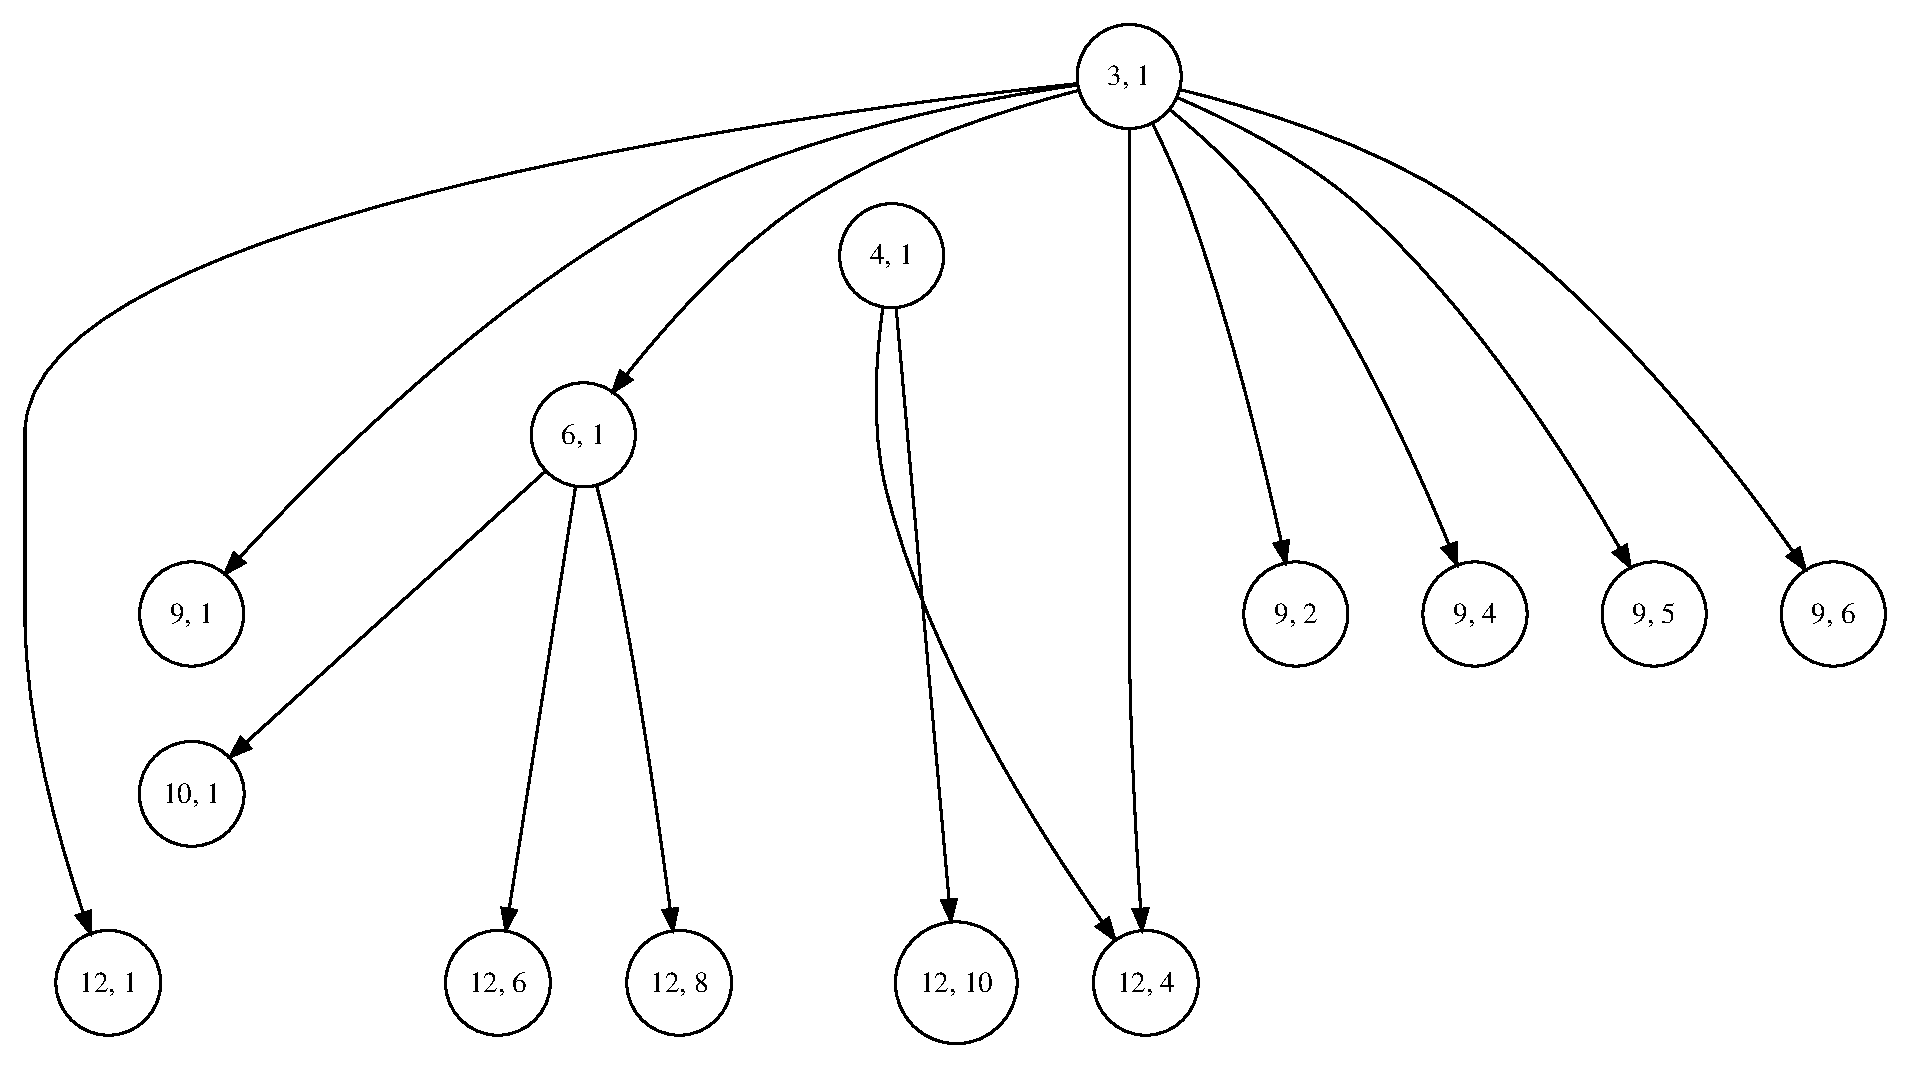
\includegraphics[scale = 0.3]{Thesis/images/SubQuandle1.eps}
    \caption{Subquandles graph}
    \label{fig:my_label}
\end{figure}
\end{frame}

\begin{frame}{Applications 2/3}
\begin{figure}[H]
    \centering
    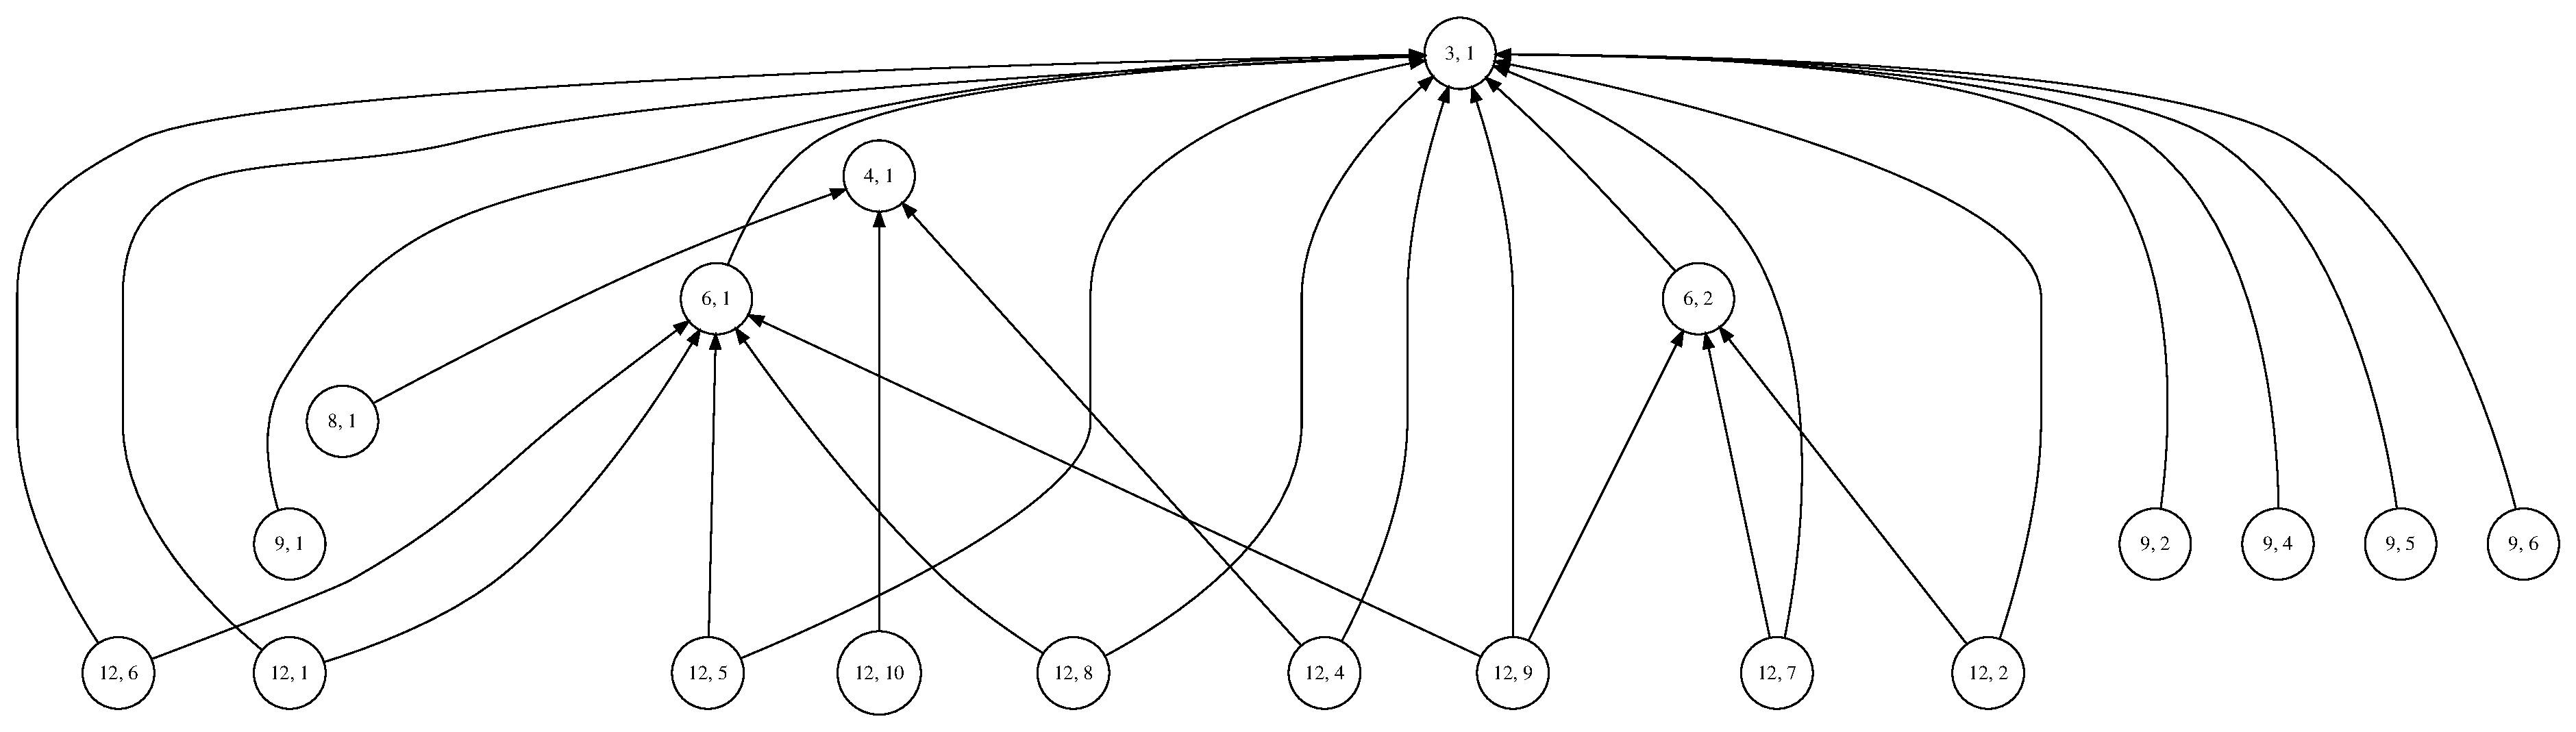
\includegraphics[scale = 0.19]{Thesis/images/BigConnectedQuoQuandle.eps}
    \caption{Quotient quandles graph}
    \label{fig:my_label}
\end{figure}
\end{frame}



\begin{frame}{Applications 3/3}
\small
\begin{columns}
\begin{column}{0.3\textwidth}

\begin{figure}[H]
    \centering
    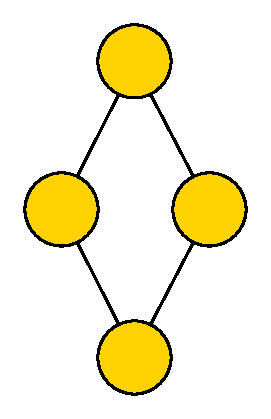
\includegraphics[scale = 0.5]{Thesis/images/Coloured28_2LatticeGraph.eps}
    \caption{Congruence Lattice \\ Subdirectly reducible}
    \label{fig:my_label}
\end{figure}
Direct product of strictly simple quandles (quandles with no proper subquandles).
\end{column}
\begin{column}{0.3\textwidth}

\begin{figure}[H]
    \centering
    \includegraphics[scale = 0.5]{Thesis/images/Coloured28_3LatticeGraph.eps}
    \caption{Congruence Lattice  \\ Subdirectly irreducible}
    \label{fig:my_label}
\end{figure}

\end{column}
\begin{column}{0.3\textwidth}

\begin{figure}[H]
    \centering
    \includegraphics[scale = 0.5]{Thesis/images/Coloured3_1LatticeGraph.eps}
    \caption{Congruence Lattice \\ Simple}
    \label{fig:my_label}
\end{figure}

\end{column}
\end{columns}
\end{frame}
\begin{frame}{Applications + Some background}
\normalsize
\begin{itemize}
    \item If $Q$ is a connected quandle, then every quotient quandle is also connected\footnote{Marco Bonatto and David Stanovský. Commutator theory for racks and quandles. \emph{Journal of the Mathematical Society of Japan} 73.1 (2021): 41-75.}.
\item A congruence in which all blocks have the same size is called \emph{uniform}$^{5}$.
\item Using that every quotient quandle and the block of every proper congruence have prime size, one can show that the congruence lattice of connected quandles of size $pq$ is one of the three shown in \emph{Applications 3/3}. Every factor is strictly simple and connected, which allows the characterization of subdirectly reducible quandles of size $pq$ using Lemma 2.6 in \footnote{Marco Bonatto. Connected quandles of size $pq$ and $4p$.\emph{Osaka Journal of Mathematics} 59.1 (2022): 145-175.}.
\end{itemize}
\end{frame}
\begin{frame}{Quandles and congruences}
\normalsize
\begin{itemize}
    
\item Given a quandle $Q$ and a congruence $\alpha$ such that $Q/\alpha$ is connected. The blocks of $\alpha$ are pairwise isomorphic subquandles of $Q$. In general, the blocks of the partitions induced by a congruence relation, associated with the restriction to them of the operation of Q are subquandles.$^{5,6}$
\item Congruences of a quandle $Q$ induce a surjective homomorphism between the displacement group (and inner automorphism group) of $Q$ and the displacement group(and inner automorphism group) of its quotient quandles\footnote{Marco Bonatto. Principal and doubly homogeneous quandles. \emph{Monatshefte für Mathematik} 191.4 (2020): 691-717.}.
\end{itemize}

\end{frame}

\begin{frame}{Faster Methods 1/2}
\normalsize
For any automorphism $h$ of $Q$ and any element $x\in Q$ we have $L_{h(x)} = hL_xh^{-1}$
\footnote{David Stanovský. Left distributive left quasigroups. \emph{Diss. PhD Thesis, Charles University in Prague}, 2004.}
    
\end{frame}

\begin{frame}{Faster Methods 2/2}
\normalsize
Global invariants:\newline
A polynomial invariant of finite quandles such as the one presented in \textit{A polynomial invariant of finite quandles} by Sam Nelson.\newline\newline
Other global invariants are connected to $Inn(Q)$, for example: \newline\newline
Let us use $Nil(G)$ to indicate the nilpotency class of a group $G$:
\[A \hookrightarrow B \implies Nil(Inn(A)) \leq Nil(Inn(B)) \]
    Individual invariants:\newline
    The number of elements fixed by the left translation map corresponding to the element $x$: $|\{y \in Q : L_x(y) = y \}|$.
\end{frame}

